\section{Example Scenario}
\label{sec:Example}

\begin{figure*}
    \centering
    \begin{subfigure}[b]{0.45\textwidth}
			\centering
      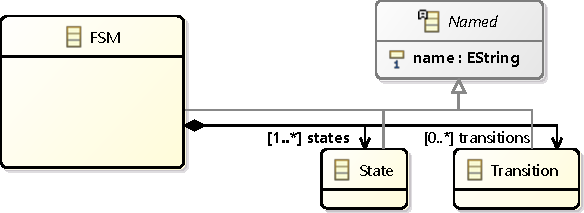
\includegraphics[width=\textwidth]{FSM0.pdf}
      \caption{Initial \metamodel.}
      \label{fig:FSM:Init}
    \end{subfigure}
    \hfill
    \begin{subfigure}[b]{0.45\textwidth}
			\centering
      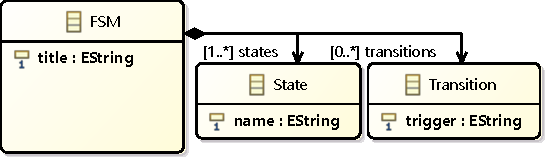
\includegraphics[width=\textwidth]{FSM1.pdf}
      \caption{\textbf{Step 1:} Specifying relevant \textsf{name}s}
      \label{fig:FSM:Relevant}
    \end{subfigure}
    \hfill
    \begin{subfigure}[b]{0.45\textwidth}
			\centering
      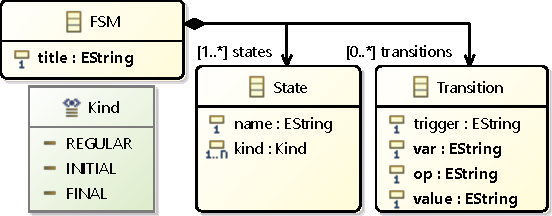
\includegraphics[width=\textwidth]{FSM2.pdf}
      \caption{\textbf{Step 2:} Adding rudimentary information for guards}
      \label{fig:FSM:Guard}
    \end{subfigure}
    \hfill 
		\begin{subfigure}[b]{0.45\textwidth}
			\centering
      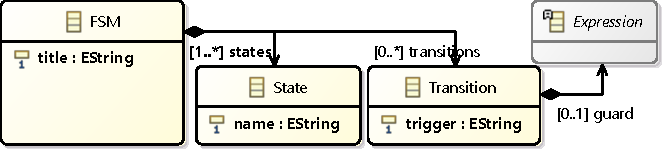
\includegraphics[width=\textwidth]{FSM3.pdf}
      \caption{\textbf{Step 3:} Specifying a fully-fledged \textsf{Expression} for \textsf{guard}s.}
      \label{fig:FSM:Expression}
    \end{subfigure}
    \caption{Three evolution steps for the \textsf{FSM} \metamodel}
    \label{fig:FSM}
\end{figure*}

\MA{Not finished yet! It needs:
\begin{itemize}
	\item Figures for views;
	\item Eventually, explanation that all is synced with the internal model.
	\item Explanation on the impact of the changes
\end{itemize}
Note that I completely failed at finding evolution steps that are purely ``atomic'':
any \emph{meaningful} (in the sense of my explanation here) evolution step, even
for such a small example, actually uses \textbf{a list of} atomic/composite 
changes!!! This was only partially discussed in our last meeting...}

This Section describes a small, yet representative example of \metamodel
evolution steps on a popular \textsc{Dsl}, the Finite State Machine (\textsf{FSM}).
Note that we simplify the \metamodels and corresponding \viewtypes, to focus 
the discussion only on the parts relevant to co-evolution. 

A methodologist starts with the simple version depicted in Figure \ref{fig:FSM:Init}:
an \textsf{FSM} consists of \textsf{State}s and \textsf{Transition}s. Each class
inherits a \textsf{name} that denotes the \textsf{FSM}'s title, the \textsf{State}'s
name, and the \textsf{Transition}'s trigger. From this initial version of \textsf{FSM},
the methodologist defines two views (types). The first one is \emph{visual},
and relies on different \textsf{Rountangle}s and \textsf{Arrow}s to depict the 
\textsf{FSM}, and provides two counters displaying the total number of \textsf{State}s
and \textsf{Transition}s in a model. The second one is \emph{textual}, and offers
a compact representation where \textsf{Transition}s are ``embedded'' inside 
\textsf{State}s. The specification, and an \textsf{FSM} model consisting of two
\textsf{State}s with three \textsf{Transition}s, are depicted in Figure \ref{fig:VT}.

In a first evolution step, the methodologist refines the \textsf{FSM} metamodel,
after noticing that the inherited \textsf{name}s actually play different functions,
by  \emph{pushing down} the \textsf{name} attribute and \emph{renaming} it where
appropriate. This evolution step does not impact the \viewtypes, but rather the
way information in views is computed: for example, displaying the \textsf{TextArea}
above an \textsf{Arrow} in the visual representation needs to be updated from
\texttt{self.name} to \texttt{self.\textbf{trigger}}. 

In a second evolution step, the methodologist wants to extend \textsf{FSM}'s 
behaviour by adding a rudimentary representation for guards that may prevent
triggering a \textsf{Transition} when evaluated to \texttt{false}. For this purpose,
three new attributes are \emph{created} in \textsf{Transition}, allowing to capture
simple expressions over \textsf{var}iables, using boolean and numeric \textsf{value}s
(e.g. \textsf{v = 10} or \textsf{k or l}). After that, \textsf{FSM}'s views, as 
depicted in Fig. \ref{fig:VT}, may still be valid wrt. the evolved \metamodel 
(assuming the lack of guard is interpreted as a trivial \textsf{true} guard),
but \viewtypes still need to reflect this new information by \emph{ADD}ing new 
entities. 

In a final evolution step, the methodologist, confident with the implemented
execution engine, specifies a fully-fledged \textsf{Expression} model,
allowing a \textsf{Transition} to possess a \textsf{guard}, thus \emph{deleting}
the extra attributes added in the previous step.


\begin{figure*}
    \centering
    \begin{subfigure}[b]{0.45\textwidth}
			\centering
      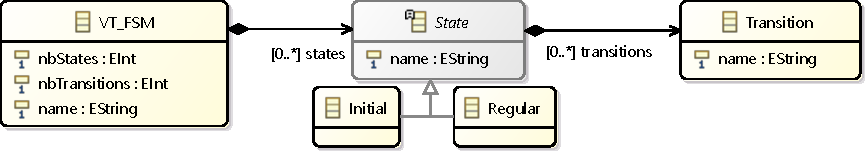
\includegraphics[width=\textwidth]{FSM_VT.pdf}
      \caption{Viewtype for the \emph{visual} representation}
      \label{fig:VT:VMM}
    \end{subfigure}
    \hfill
    \begin{subfigure}[b]{0.45\textwidth}
			\centering
      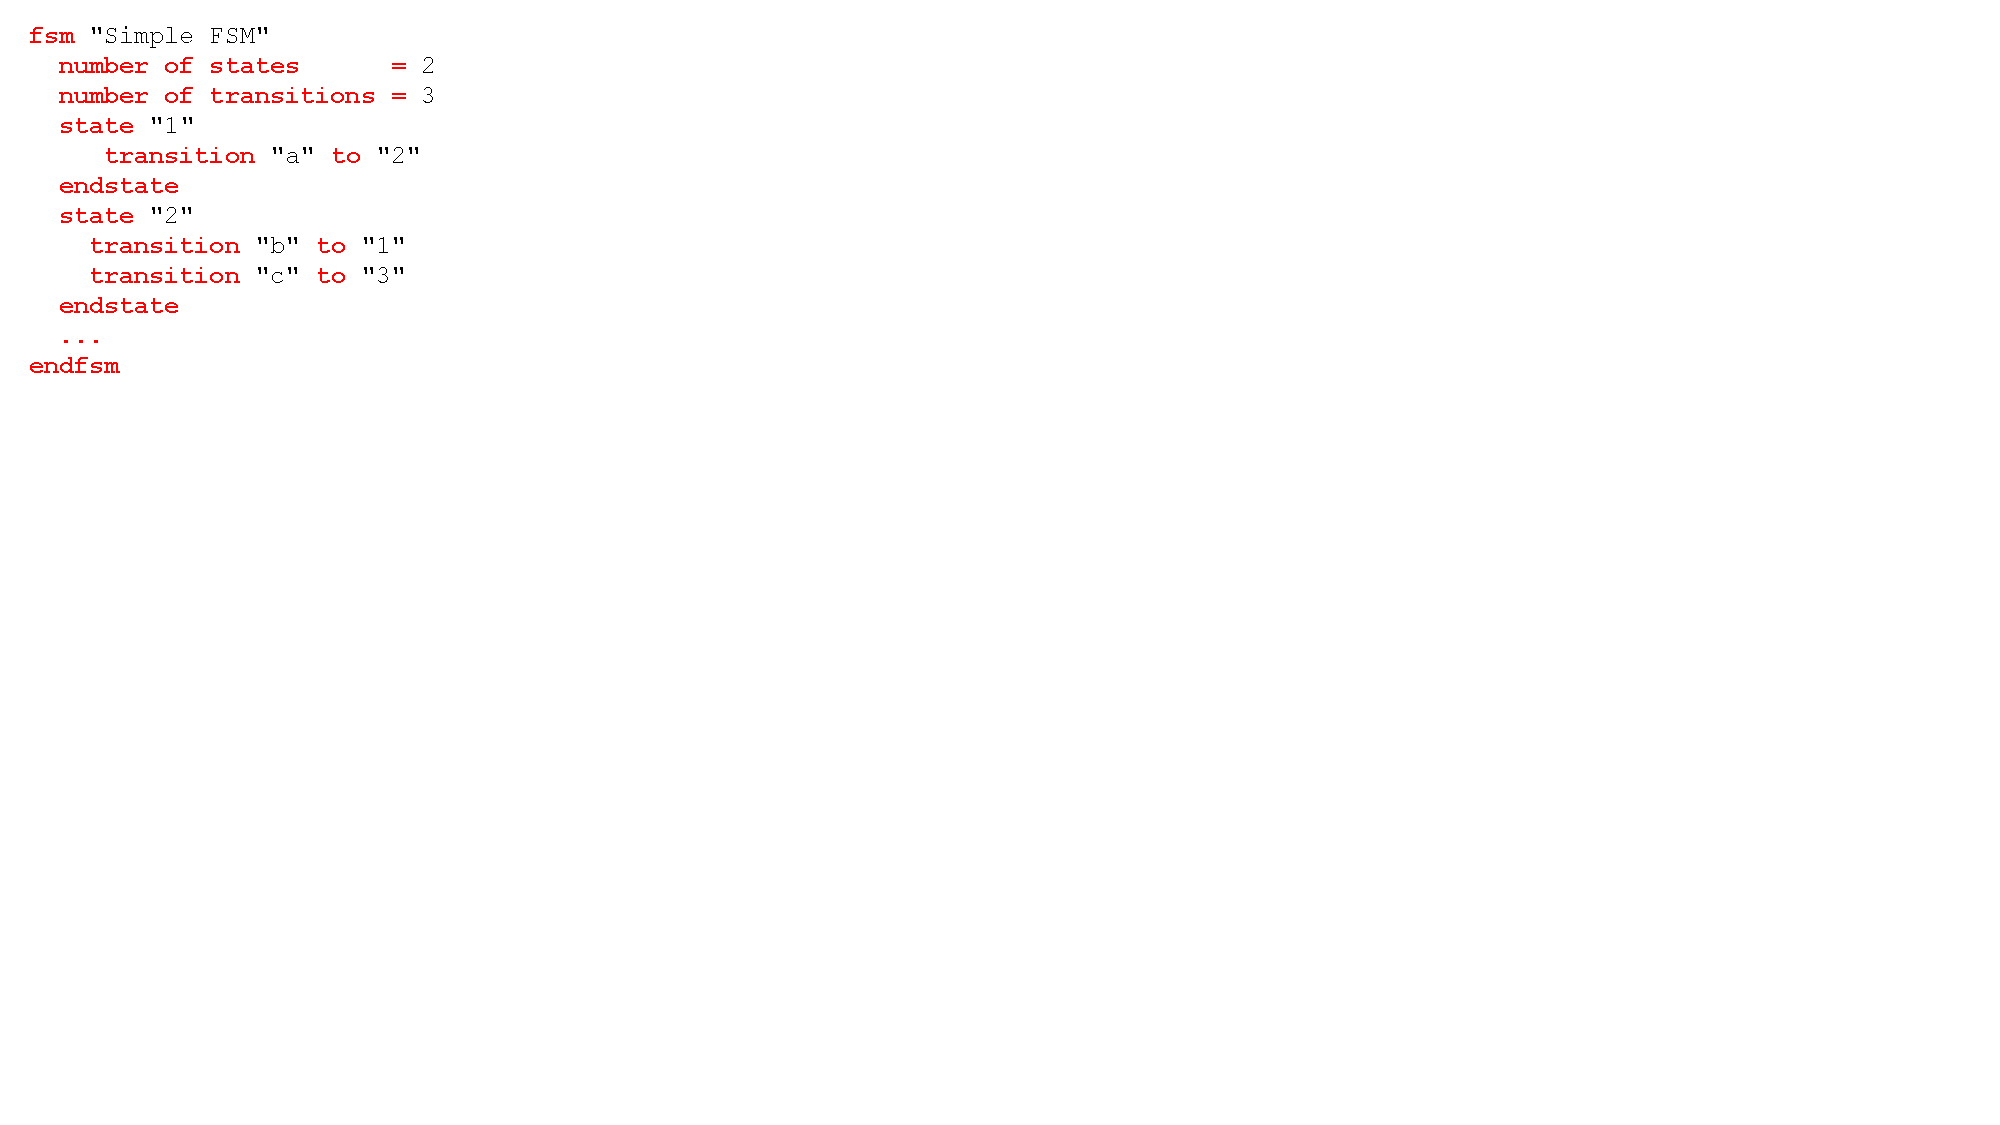
\includegraphics[width=0.65\textwidth, page=1, clip, trim=0cm 11.6cm 21.4cm 0cm]{VT.pdf}
      \caption{A \textsf{Simple FSM} model conforming to the \emph{visual} \viewtype}
      \label{fig:VT:VM}
    \end{subfigure}
    \hfill
    \begin{subfigure}[b]{0.45\textwidth}
			\centering
      \includegraphics[width=0.6\textwidth, page=2, clip, trim=0cm 14cm 26cm 0cm]{VT.pdf}
      \caption{Viewtype for the \emph{textual} representation \MA{Write the BNF spec!}}
      \label{fig:VT:TMM}
    \end{subfigure}
    \hfill
    \begin{subfigure}[b]{0.45\textwidth}
			\centering
      \includegraphics[width=0.6\textwidth, page=2, clip, trim=0cm 13.5cm 26cm 0cm]{VT.pdf}
      \caption{A \textsf{Simple FSM} model conforming to the \emph{textual} \viewtype}
      \label{fig:VT:TM}
    \end{subfigure}
    \caption{Two \viewtypes, and associated views depicted the \textsf{Simple FSM} model.}
    \label{fig:VT}
\end{figure*}
